\chapter[Experimentos e Resultados]{Experimentos e Resultados} \label{cap:resultados}
    Para testar o pacote \textit{rqt\_mrta}, será necessário uma arquitetura desenvolvida sobre o \textit{framework} ROS. Primeiramente, será necessário compreendê-la e entender como parametrizá-la. A partir disso, será possível estruturar os \textit{templates} de arquivos de configuração e de inicialização, isto é, criar seu arquivo de configuração, conforme descrito em \ref{subsec:arch_config_fmt}. Tendo este arquivo em mãos, é preciso alterar o arquivo manifesto do seu pacote para que a configuração possa ser vista pelo \textit{rqt\_mrta}. Este processo foi descrito em \ref{subsec:arch_config_rgst}. Finalmente, a arquitetura estará cadastrada e pronta para ser configurada por usuários na criação de aplicações.
    
    Além de uma arquitetura, será necessário a elaboração de uma aplicação que utilize a arquitetura cadastrada. Pois, assim, será validado o processo de criação da aplicação. Isto é, deverá ser verificado se o pacote da nova aplicação foi gerado com sucesso. Para isso, deve se verificar se ele é visível pelas ferramentas de busca do ROS e se a formatação dos arquivos de parâmetro, de inicialização e de configuração de aplicação está correta. Se tudo estiver em conformidade, então aplicação estará pronta para a execução. É preciso, agora, executar a aplicação utilizando os arquivos de inicialização gerados pelo \textit{rqt\_mrta}. Para isso, será utilizada a ferramenta \textit{roslaunch} para a inicialização dos nós da aplicação. 
    
    Finalmente, será verificado o sistema supervisório do \textit{rqt\_mrta}. Para isso, a aplicação deverá ser carregada pelo \textit{rqt\_mrta}, o qual ficará aguardando a aplicação ser executada. Nesta etapa será verificada a alteração do estado dos robôs no sistema e, se fornecido, a inicialização do \textit{plugin} para o monitoramento da arquitetura.
    
    Pelo fato de haver poucas aproximações genéricas de arquitetura MRTA para aplicações baseadas em ROS, foi desenvolvido o pacote \textit{alliance}. Esse pacote faz uma aproximação independente do domínio da arquitetura tolerante à falhas ALLIANCE \cite{ref:parker1998alliance} para atribuição de tarefa em sistema multirrobô. Esta arquitetura será utilizada para testar o funcionamento do pacote \textit{rqt\_mrta}. 
    
    Será criado, através do \textit{rqt\_mrta}, uma aplicação que utilize a arquitetura desenvolvida no pacote \textit{alliance} para a atribuição de tarefa no sistema. Será simulado a patrulha realizada por múltiplos robôs.
    
    A seguir será descrito o desenvolvimento da arquitetura ALLIANCE no pacote \textit{alliance}. Em seguida, está arquitetura será cadastrada para sua utilização por aplicações no \textit{rqt\_mrta}. Depois, a aplicação será explicada e criada através do \textit{rqt\_mrta}. Por fim, os arquivos de inicialização da arquitetura serão executados em conjunto com o simulador e os demais nós para a execução da aplicação.

    \section{\textit{alliance}} \label{sec:alliance}
        O \textit{alliance} é um projeto baseado em ROS que contém nós que fazem o controle distribuído da alocação de tarefa em um sistema com múltiplos robôs segundo o modelo sugerido por \citeonline{ref:parker1998alliance}, a arquitetura ALLIANCE. 
            
        O Apêndice \ref{app:alliance} dá mais detalhes sobre o funcionamento da arquitetura ALLIANCE.
        
        \subsection{\textit{alliance\_msgs}}
            O pacote \textit{alliance\_msgs} foi criado em conjunto com o pacote \textit{alliance} para separar as definições dos tipos de mensagens utilizadas por ele. Essas mensagens são utilizadas na comunicação entre os nós do pacote \textit{alliance}.
            
            Este pacote define as seguintes mensagens:
            
            \begin{itemize}
                \item \textit{alliance\_msgs/InterRobotCommunication}: armazena informação sobre a atividade de um robô específico em um dado instante. Possui o cabeçalho padrão do ROS que identifica o robô que enviou a mensagem e instante que ela foi enviada. Além disso, ela possui um campo que identifica a tarefa que o robô está executando;
                \item \textit{alliance\_msgs/Motivation}: utilizada para o monitoramento da arquitetura. Esta mensagem possui i cabeçalho padrão do ROS que identifica o robô que enviou a mensagem e também o instante que ela foi enviada. Além disso, ela possui um campo que identifica a tarefa que o cálculo de motivação se referencia e, ainda, o valor das variáveis que influenciam no cálculo da motivação;
                \item \textit{alliance\_msgs/SensoryFeedback}: utilizada na comunicação entre os nós de baixo e alto nível de abstração de um mesmo robô. Esta mensagem informa se um dado comportamento é aplicável em um dado instante segundo uma análise sensorial realizada no nível de baixa abstração do \textit{alliance}. Assim está mensagem possui o cabeçalho padrão do ROS que identifica o robô que enviou a mensagem e instante que ela foi enviada. Além disso, ela possui um campo que identifica a tarefa que a análise está referenciada e, ainda, um campo informando se a ativação do comportamento que leva esse robô a executar essa tarefa é aplicável.
            \end{itemize}
        
        \subsection{\textit{rqt\_alliance}}
            O pacote \textit{rqt\_alliance} foi desenvolvido para auxiliar no monitoramento da arquitetura implementada no pacote \textit{alliance}. Ele fornece uma ferramenta gráfica que mostra o nível de motivação de cada robô em tempo de execução. Esta interface também fornece gráficos que detalham as variáveis que influenciam no cálculo de motivação de uma configuração de comportamento de um robô específico.
            
            \begin{figure}
                \centering
                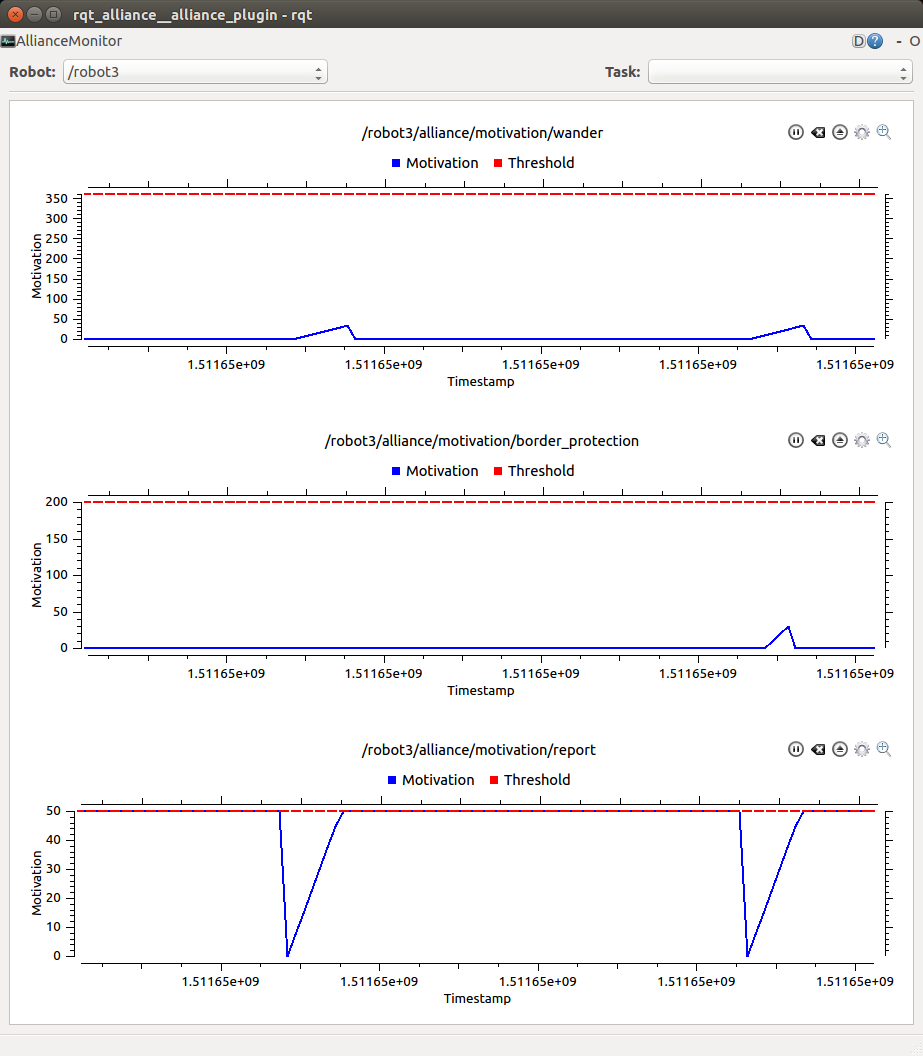
\includegraphics[width=\textwidth]{Figuras/4_resultados/rqt_alliance4.png}
                \caption{Motivações das configurações de comportamento do robô \textit{/robot3}.}
                \label{fig:rqt_alliance_motivations}
            \end{figure}
            
            \begin{figure}
                \centering
                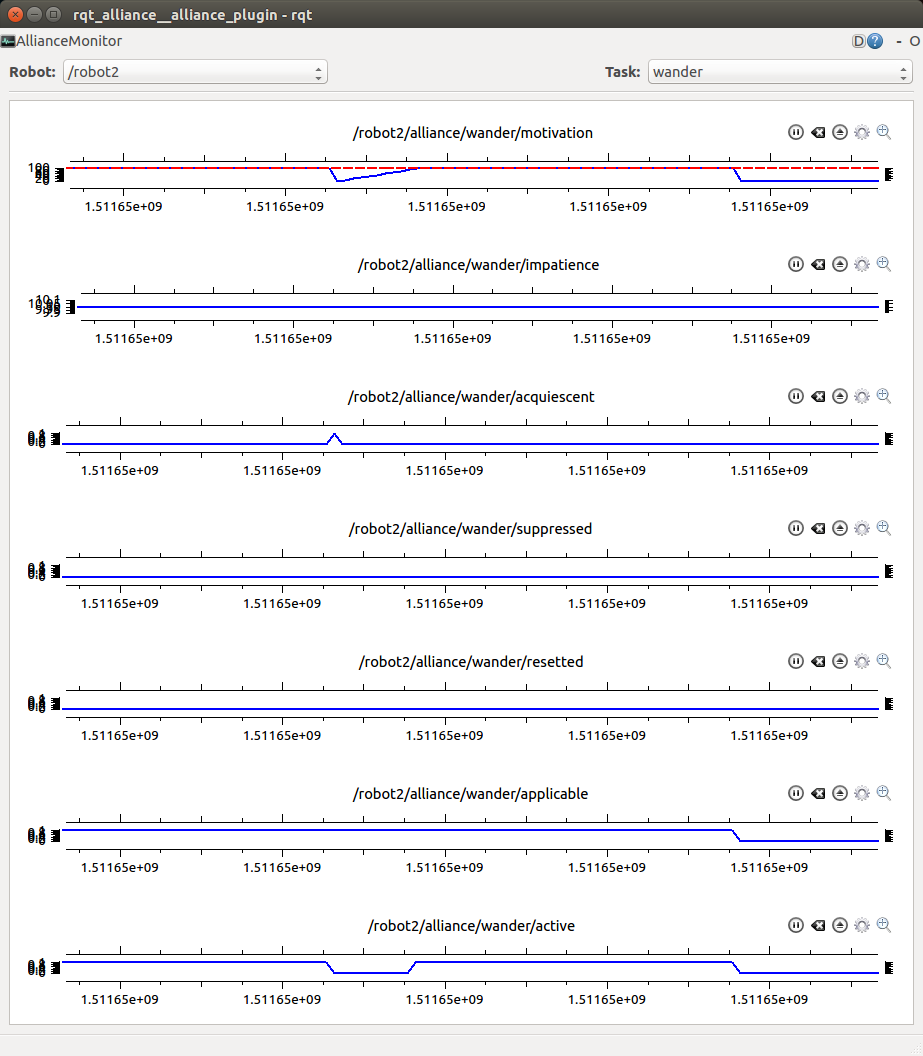
\includegraphics[width=\textwidth]{Figuras/4_resultados/rqt_alliance6.png}
                \caption{Detalhamento da motivação \textit{/robot2/alliance/wander} ao longo do tempo.}
                \label{fig:rqt_alliance_detailed_motivation}
            \end{figure}
        
    \section{\textit{patrulha}}
        
        \begin{figure}[htb]
            \centering
            \subfloat[Dados gerais da aplicação.]{
                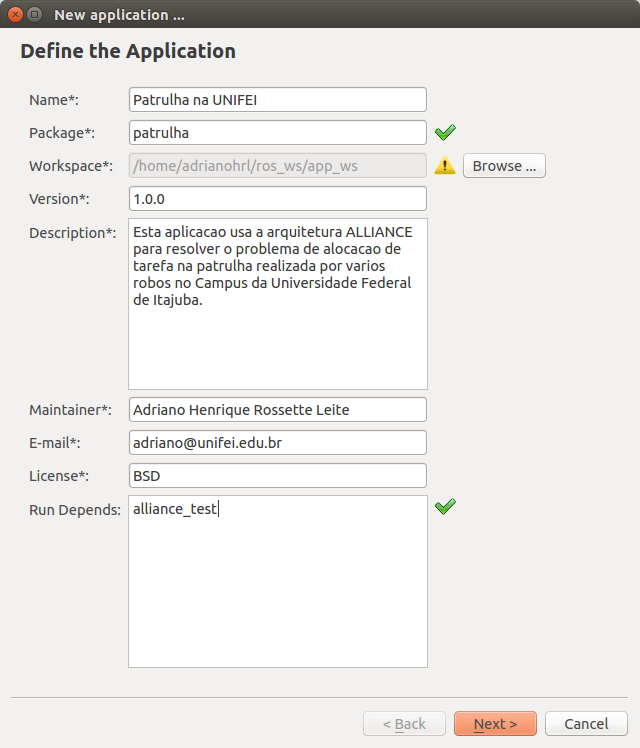
\includegraphics[width=.31\textwidth]{Figuras/4_resultados/patrulha_def_app.png}
                \label{fig:patrulha_def_app}
            }
            \subfloat[Escolha da arquitetura.]{
                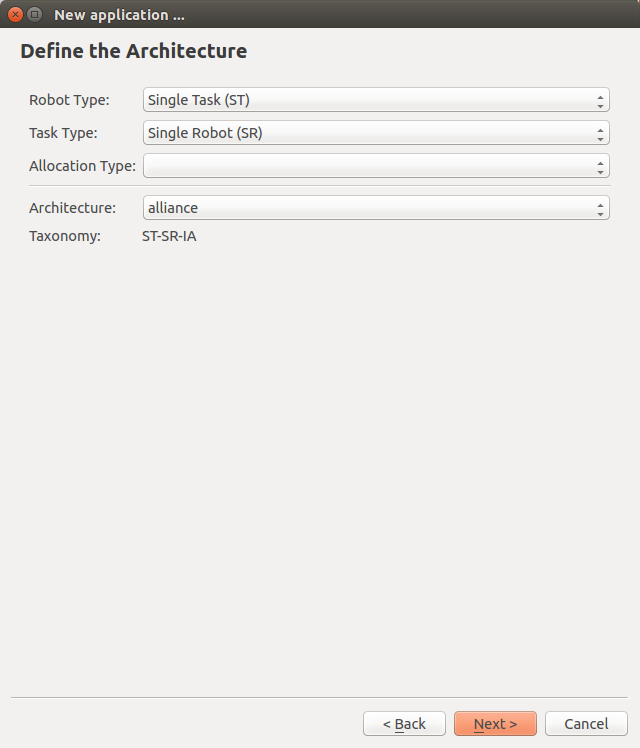
\includegraphics[width=.31\textwidth]{Figuras/4_resultados/patrulha_def_arch.png}
                \label{fig:patrulha_def_arch}
            }
            \subfloat[Definição dos robôs do sistema.]{
                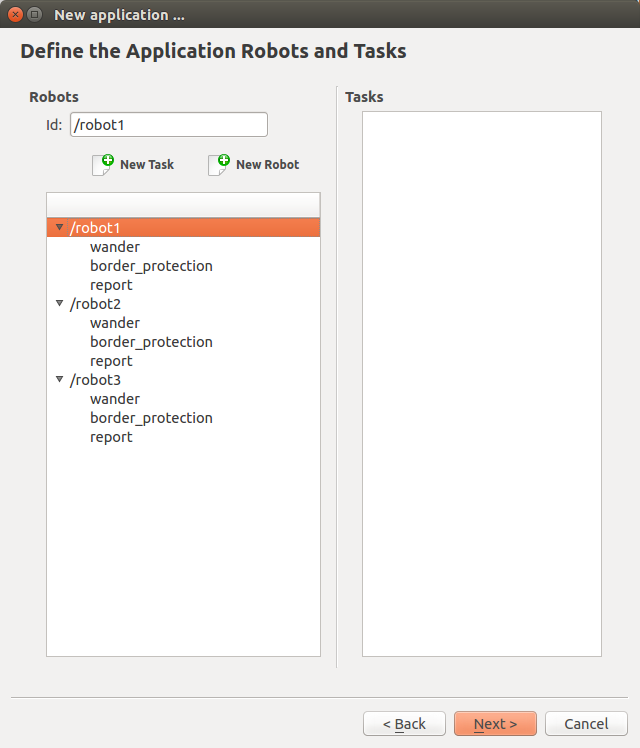
\includegraphics[width=.31\textwidth]{Figuras/4_resultados/patrulha_def_robots.png}
                \label{fig:patrulha_def_robots}
            }
            
            \subfloat[Parametrização da arquitetura.]{
                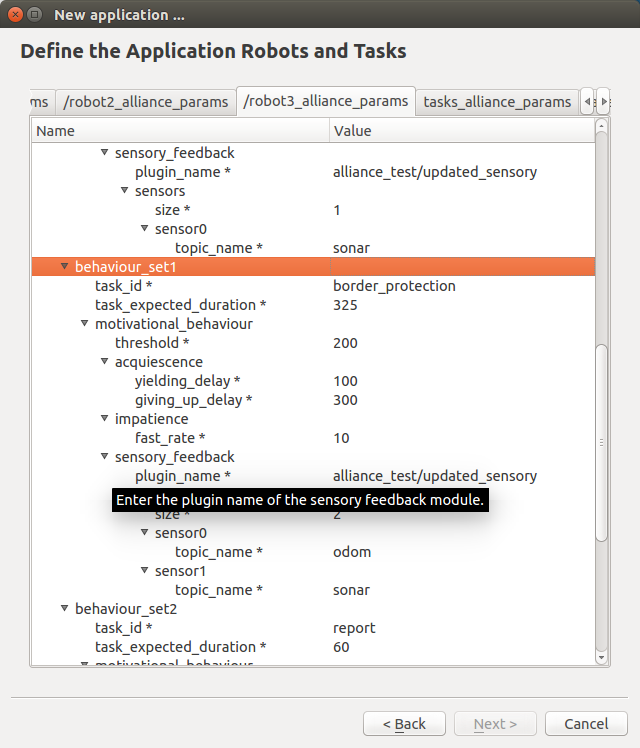
\includegraphics[width=.31\textwidth]{Figuras/4_resultados/patrulha_def_params.png}
                \label{fig:patrulha_def_params}
            }
            \subfloat[Sumário.]{
                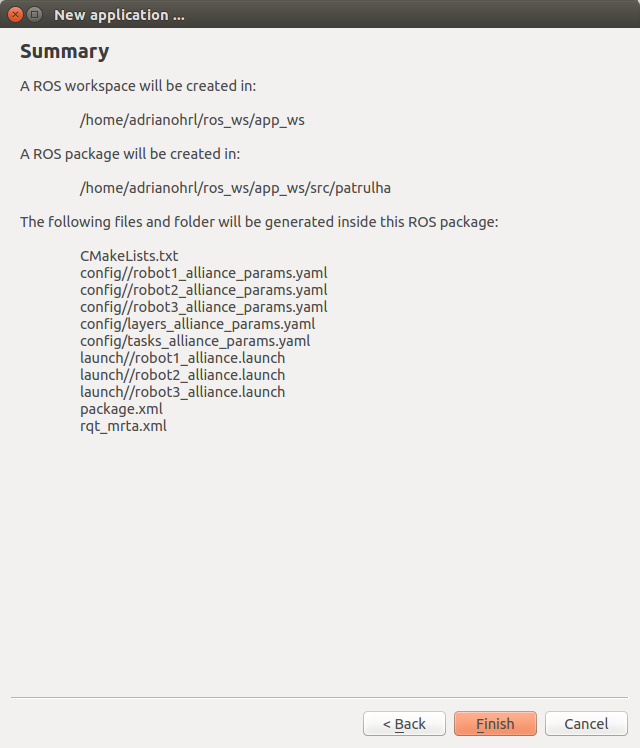
\includegraphics[width=.31\textwidth]{Figuras/4_resultados/patrulha_summary.png}
                \label{fig:patrulha_summary}
            }
            \caption{Criação da aplicação \textit{patrulha}.} \label{fig:patrulha_new_app}
        \end{figure}
        
        \begin{figure}[htb]
            \centering
            \subfloat[Pacote.]{
                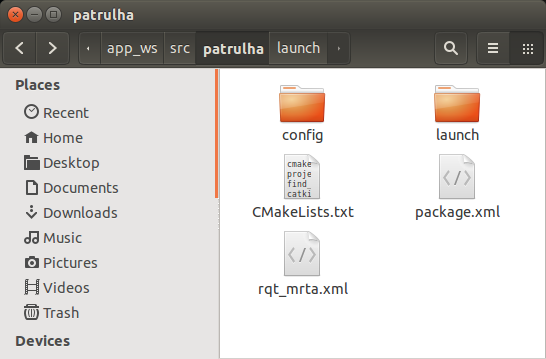
\includegraphics[width=.4\textwidth]{Figuras/4_resultados/patrulha_pkg.png}
                \label{fig:patrulha_pkg}
            }
            \subfloat[Arquivos de parâmetro.]{
                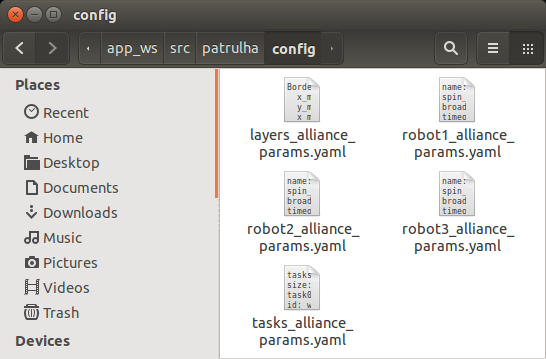
\includegraphics[width=.4\textwidth]{Figuras/4_resultados/patrulha_pkg_config.png}
                \label{fig:patrulha_pkg_config}
            }
            
            \subfloat[Arquivos de inicialização.]{
                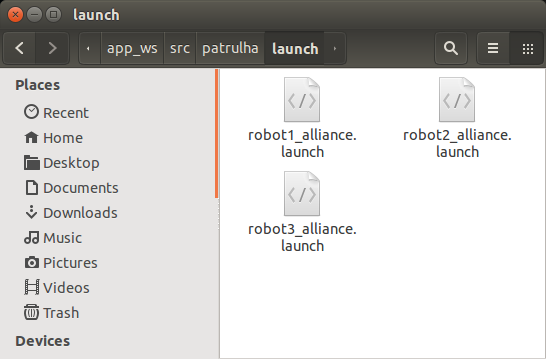
\includegraphics[width=.4\textwidth]{Figuras/4_resultados/patrulha_pkg_launch.png}
                \label{fig:patrulha_pkg_launch}
            }
            \caption{Pastas e arquivos gerados após a criação de uma aplicação.} \label{fig:patrulha}
        \end{figure}
        
        
        \begin{figure}[p]
            \centering
            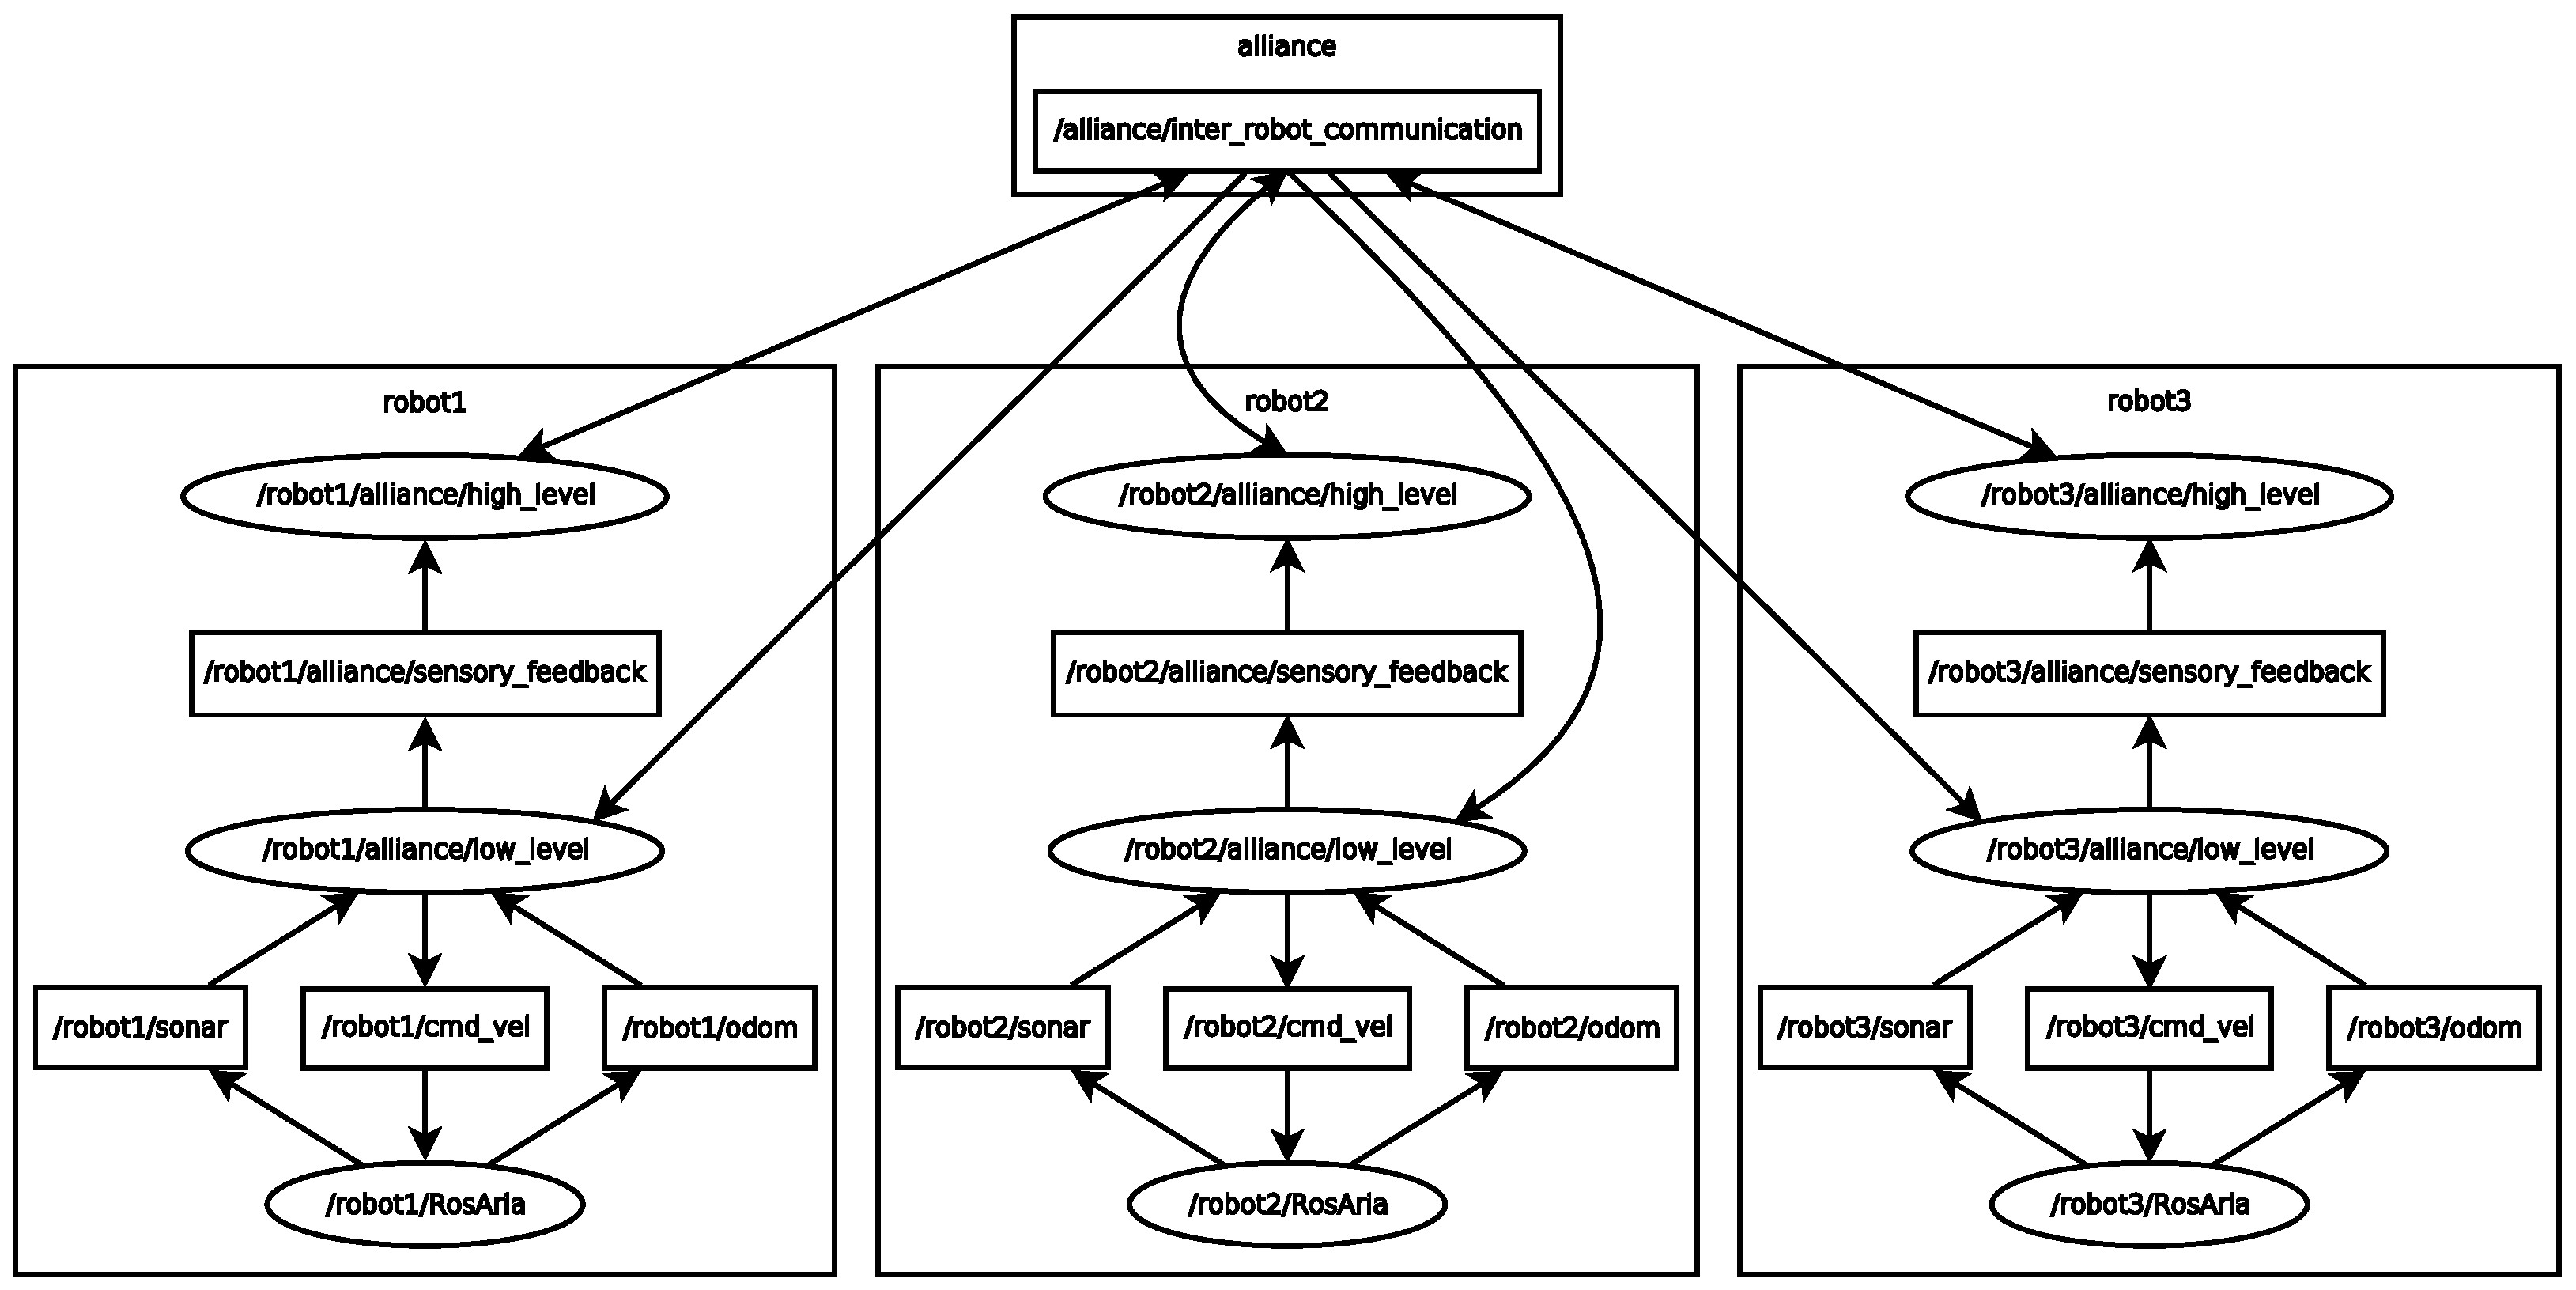
\includegraphics[width=.97\textheight,angle=90]{Figuras/4_resultados/rosgraph_3robots.eps}
            \caption{Grafo do ALLIANCE no ROS para três robôs.} \label{fig:ros_graph_alliance}
        \end{figure}
        
        
    
        \pgfplotstableread[col sep=comma]{\detokenize{Figuras/capitulo_3/robot1-wander-motivation-new.csv}}\datatable
\begin{figure}[htb]
    \centering
    \begin{tikzpicture}
    \begin{groupplot}[
      group style={rows=6}, 
      width=0.75\textwidth,
      height=0.25\textwidth, 
      xmajorgrids, 
      ymajorgrids, 
      enlarge x limits=false,
    ] 
        \nextgroupplot[
        %title={Motivação da configuração de comportamento /robot1/wander.},
        ymin=-0.1,
        ylabel={$impaci\hat{e}ncia(t)$},
        ]
        \addplot[blue,line width=1pt] table[x index=0,y index=1]{\datatable}; 
        
        \nextgroupplot[
        ymin=-0.1,
        ymax=1.1,
        ylabel={$aquiescente(t)$},
        ] 
        \addplot[blue,line width=1pt] table[x index=0,y index=2]{\datatable}; 
        
        \nextgroupplot[
        ymin=-0.1,
        ymax=1.1,
        ylabel={$inibida(t)$},
        ] 
        \addplot[blue,line width=1pt] table[x index=0,y index=3]{\datatable}; 
        
        \nextgroupplot[
        ymin=-0.1,
        ymax=1.1,
        ylabel={$reiniciada(t)$},
        ] 
        \addplot[blue,line width=1pt] table[x index=0,y index=4]{\datatable}; 
        
        \nextgroupplot[
        ymin=-0.1,
        ymax=1.1,
        ylabel={$aplic\acute{a}vel(t)$},
        ] 
        \addplot[blue,line width=1pt] table[x index=0,y index=5]{\datatable};
        
        \nextgroupplot[
        ylabel={$motiva\textit{ç}\tilde{a}o(t)$},
        xlabel={$t [s]$}
        ] 
        \addplot[blue,line width=1pt] table[x index=0,y index=6]{\datatable};
    \end{groupplot}
\end{tikzpicture}
    \caption{Motivação da configuração de comportamento /robot1/wander.} \label{fig:motivacao1}
\end{figure}

\pgfplotstableread[col sep=comma]{\detokenize{Figuras/capitulo_3/robot2-wander-motivation-new.csv}}\datatable
\begin{figure}[htb]
    \centering
    \begin{tikzpicture}
    \begin{groupplot}[
      group style={rows=6}, 
      width=0.75\textwidth,
      height=0.25\textwidth, 
      xmajorgrids, 
      ymajorgrids, 
      enlarge x limits=false,
    ] 
        \nextgroupplot[
        %title={Motivação da configuração de comportamento /robot1/wander.},
        ymin=-0.1,
        ylabel={$impaci\hat{e}ncia(t)$},
        ]
        \addplot[blue,line width=1pt] table[x index=0,y index=1]{\datatable}; 
        
        \nextgroupplot[
        ymin=-0.1,
        ymax=1.1,
        ylabel={$aquiescente(t)$},
        ] 
        \addplot[blue,line width=1pt] table[x index=0,y index=2]{\datatable}; 
        
        \nextgroupplot[
        ymin=-0.1,
        ymax=1.1,
        ylabel={$inibida(t)$},
        ] 
        \addplot[blue,line width=1pt] table[x index=0,y index=3]{\datatable}; 
        
        \nextgroupplot[
        ymin=-0.1,
        ymax=1.1,
        ylabel={$reiniciada(t)$},
        ] 
        \addplot[blue,line width=1pt] table[x index=0,y index=4]{\datatable}; 
        
        \nextgroupplot[
        ymin=-0.1,
        ymax=1.1,
        ylabel={$aplic\acute{a}vel(t)$},
        ] 
        \addplot[blue,line width=1pt] table[x index=0,y index=5]{\datatable};
        
        \nextgroupplot[
        ylabel={$motiva\textit{ç}\tilde{a}o(t)$},
        xlabel={$t [s]$}
        ] 
        \addplot[blue,line width=1pt] table[x index=0,y index=6]{\datatable};
    \end{groupplot}
\end{tikzpicture}
    \caption{Motivação da configuração de comportamento /robot2/wander.} \label{fig:motivacao2}
\end{figure}

\pgfplotstableread[col sep=comma]{\detokenize{Figuras/capitulo_3/robot2-border-protection-motivation-new.csv}}\datatable
\begin{figure}[htb]
    \centering
    \begin{tikzpicture}
    \begin{groupplot}[
      group style={rows=6}, 
      width=0.75\textwidth,
      height=0.25\textwidth, 
      xmajorgrids, 
      ymajorgrids, 
      enlarge x limits=false,
    ] 
        \nextgroupplot[
        %title={Motivação da configuração de comportamento /robot1/wander.},
        ymin=-0.1,
        ylabel={$impaci\hat{e}ncia(t)$},
        ]
        \addplot[blue,line width=1pt] table[x index=0,y index=1]{\datatable}; 
        
        \nextgroupplot[
        ymin=-0.1,
        ymax=1.1,
        ylabel={$aquiescente(t)$},
        ] 
        \addplot[blue,line width=1pt] table[x index=0,y index=2]{\datatable}; 
        
        \nextgroupplot[
        ymin=-0.1,
        ymax=1.1,
        ylabel={$inibida(t)$},
        ] 
        \addplot[blue,line width=1pt] table[x index=0,y index=3]{\datatable}; 
        
        \nextgroupplot[
        ymin=-0.1,
        ymax=1.1,
        ylabel={$reiniciada(t)$},
        ] 
        \addplot[blue,line width=1pt] table[x index=0,y index=4]{\datatable}; 
        
        \nextgroupplot[
        ymin=-0.1,
        ymax=1.1,
        ylabel={$aplic\acute{a}vel(t)$},
        ] 
        \addplot[blue,line width=1pt] table[x index=0,y index=5]{\datatable};
        
        \nextgroupplot[
        ylabel={$motiva\textit{ç}\tilde{a}o(t)$},
        xlabel={$t [s]$}
        ] 
        \addplot[blue,line width=1pt] table[x index=0,y index=6]{\datatable};
    \end{groupplot}
\end{tikzpicture}
    \caption{Motivação da configuração de comportamento /robot2/border-protection.} \label{fig:motivacao3}
\end{figure}